\documentclass{article}

\usepackage{graphicx}
\usepackage{tikz}
\usepackage{tikzsymbols}
\usetikzlibrary{calc,patterns,shapes.geometric}
\pagestyle{empty}
\usepackage[margin=0pt]{geometry}
\geometry{papersize={14in,12in}}

\def\centerarc[#1](#2)(#3:#4:#5){\draw[#1] ($(#2)+({#5*cos(#3)},{#5*sin(#3)})$) arc (#3:#4:#5);}

\begin{document}
	\begin{figure}
		\centering
		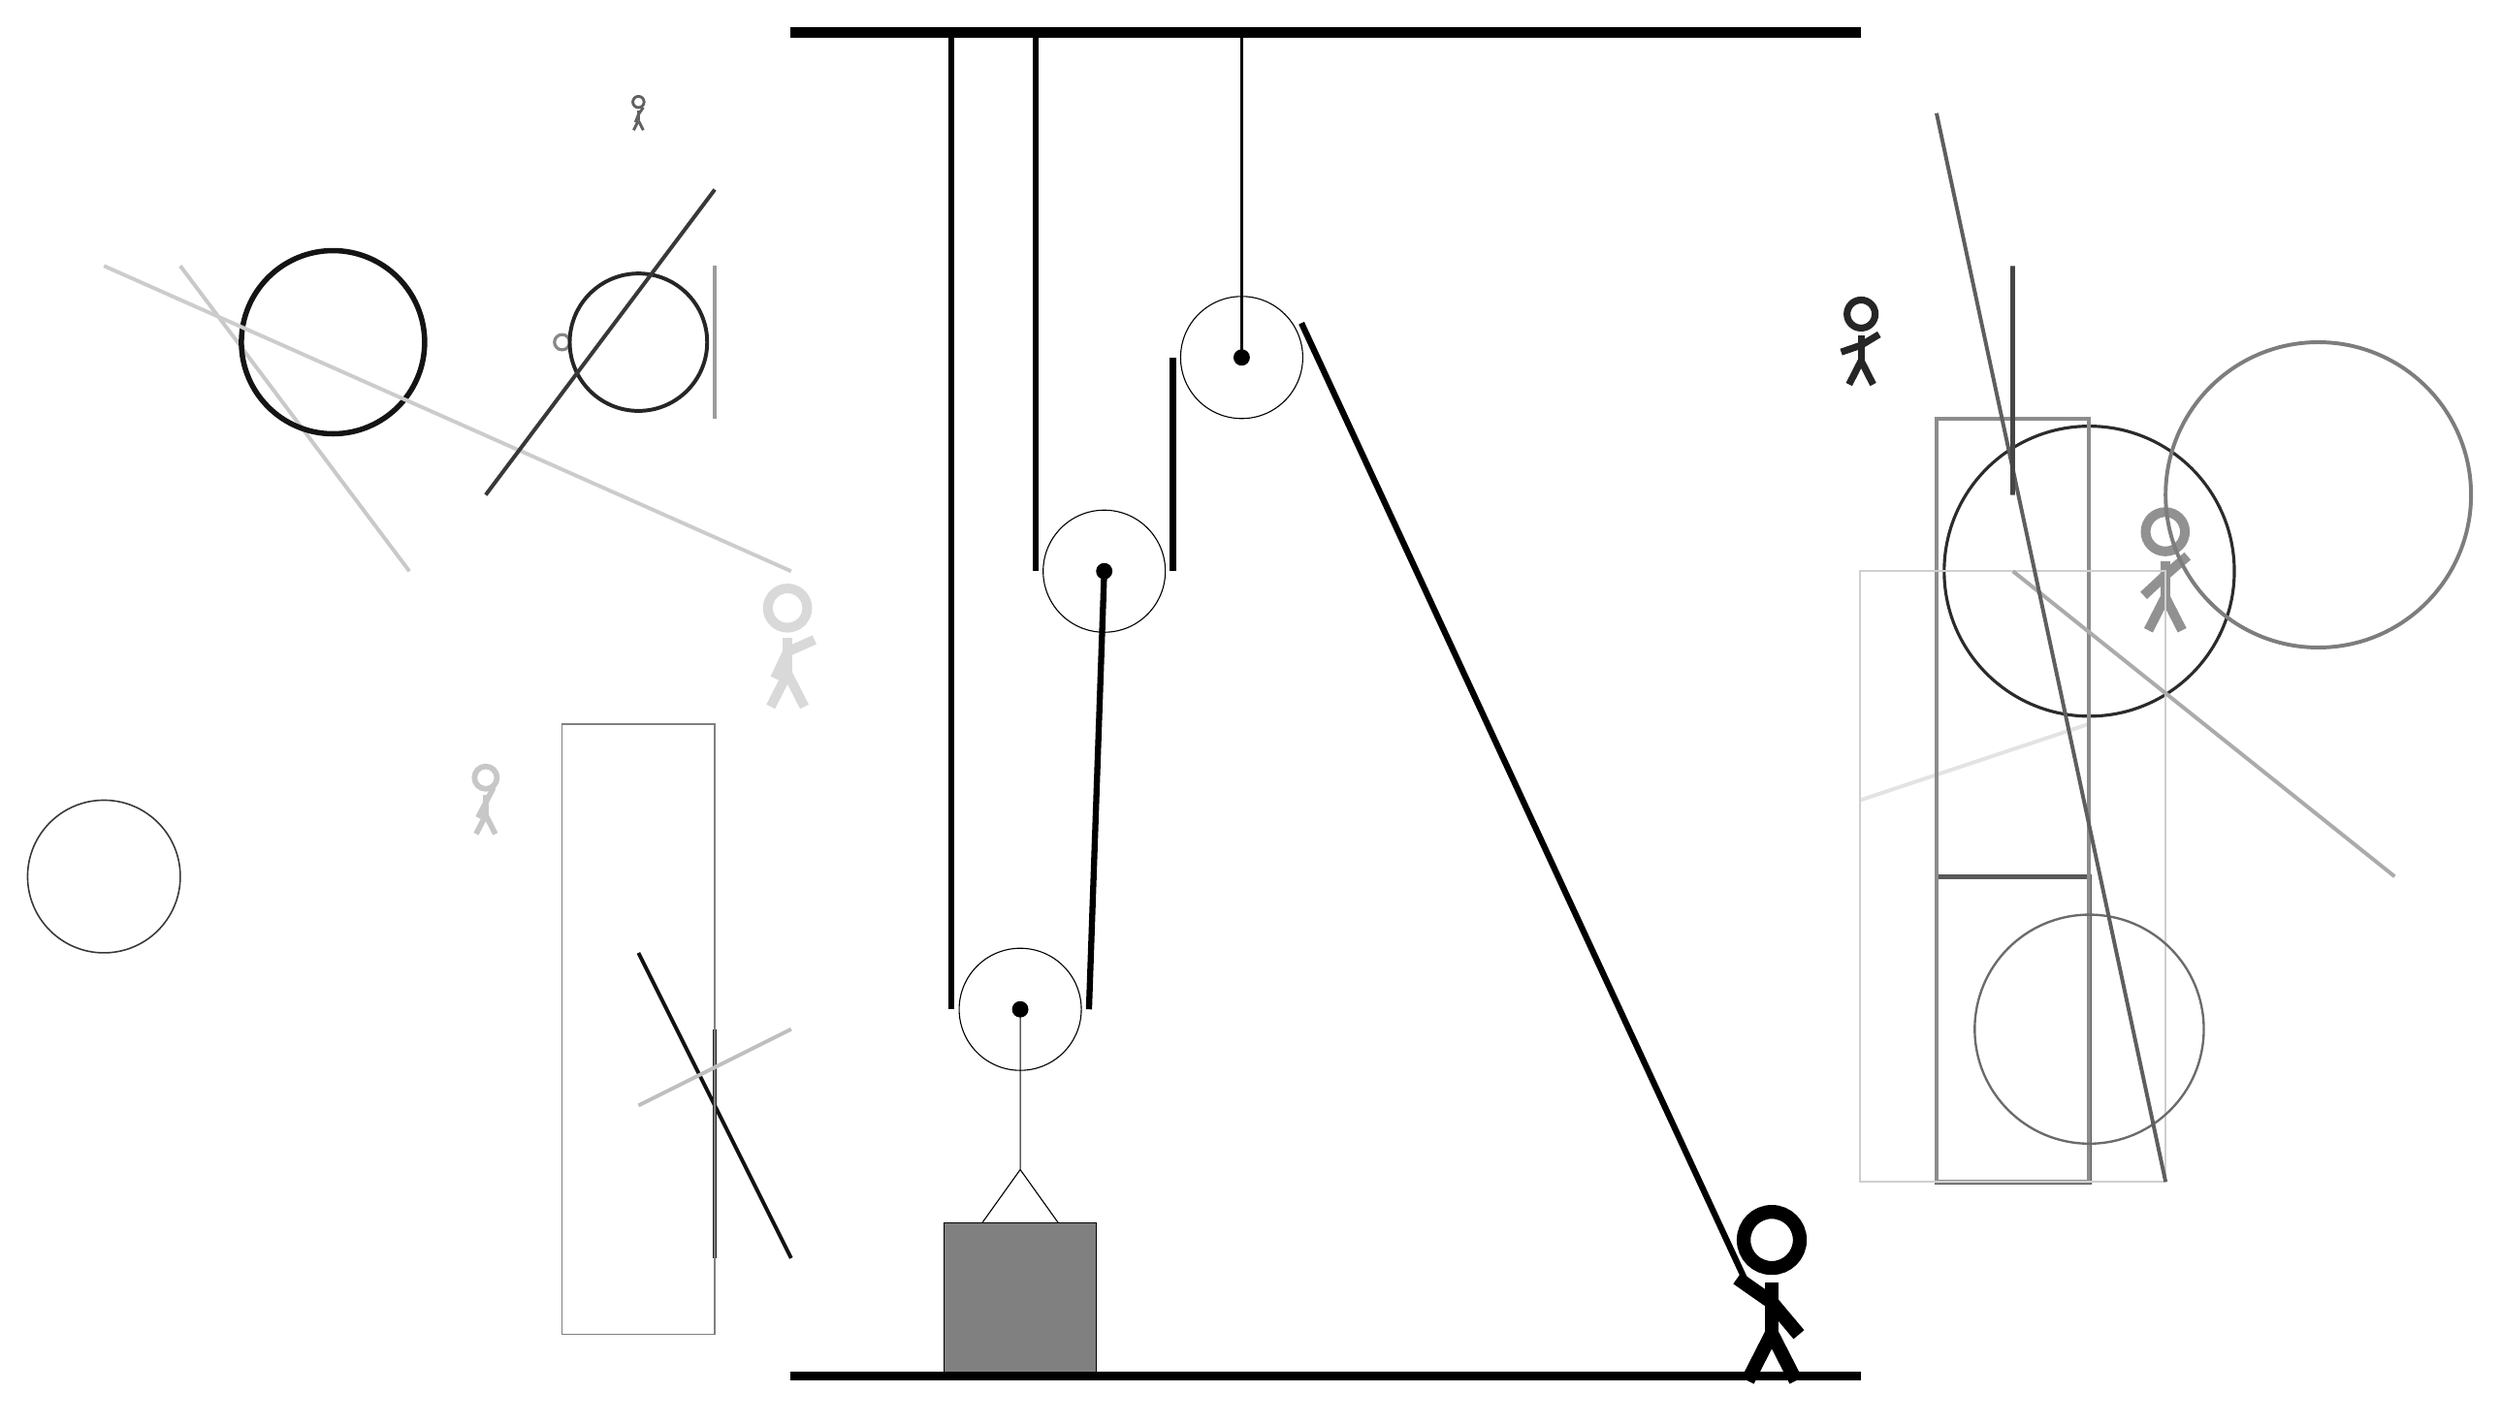
\begin{tikzpicture}
			%%%%% START %%%%%
			
			\draw[fill=black] (-2, 14) rectangle (12, 14.125);
			
			\draw (1, 1.26) circle (0.8);
			\draw[fill=black] (1, 1.26) circle (0.1);
			
			\draw (2.1, 7.0) circle (0.8);
			\draw[fill=black] (2.1, 7.0) circle (0.1);
			
			\draw (3.9, 9.8) circle (0.8);
			\draw[fill=black] (3.9, 9.8) circle (0.1);
			\draw[thick] (3.9, 9.8) -- (3.9, 14);
			
			\draw (1, 1.26) -- (1, -0.84) -- (0.5, -1.54) -- (1.5, -1.54) -- (1, -0.84);
			\draw[fill=black!50] (0, -1.54) rectangle (2, -3.54);
			
			\draw[line width=0.8mm] (0.1, 14) -- (0.1, 1.26);
			\centerarc[line width=0.8mm](1, 1.26)(180:360:0.9);
			\draw[line width=0.8mm](1.9, 1.26) -- (2.1, 7.0);
			\draw[line width=0.8mm] (1.2, 14) -- (1.2, 7.0);
			\centerarc[line width=0.8mm](2.1, 7.0)(180:360:0.9);
			\draw[line width=0.8mm](3.0, 7.0) -- (3.0, 9.8);
			\centerarc[line width=0.8mm](3.9, 9.8)(30:180:0.9);
			\draw[line width=0.8mm] (4.683, 10.25) -- (10.5, -2.3);
			
			\node at (10.8, -2.5) {\Strichmaxerl[10][-35][-50]};
			
			\draw[line width=0.5mm, color=black!21](-7, 7) -- (-10, 11);
			
			\draw [line width=0.4mm, color=black!83](15, 7) circle (1.9);
			\draw[line width=0.5mm, color=black!93](-4, 2) -- (-2, -2);
			\draw[line width=0.5mm, color=black!87](-3, 1) -- (-3, -2);
			\draw[line width=0.6mm, color=black!65] (13, -1) rectangle (15, 3);
			\draw[line width=0.5mm, color=black!11](12, 4) -- (15, 5);
			\draw [line width=0.4mm, color=black!47](-5, 10) circle (0.1);
			\draw[line width=0.5mm, color=black!39](-3, 9) -- (-3, 11);
			\draw [line width=0.5mm, color=black!85](-4, 10) circle (0.9);
			
			\node[line width=0.6mm, color=black!43] at (16, 7) {\Strichmaxerl[7][43][41]};
			
			\draw[line width=0.2mm, color=black!50] (-3, -3) rectangle (-5, 5);
			
			\draw[line width=0.5mm, color=black!25](-4, 0) -- (-2, 1);
			\draw [line width=0.7mm, color=black!92](-8, 10) circle (1.2);
			
			\node[line width=0.3mm, color=black!85] at (12, 10) {\Strichmaxerl[5][19][31]};
			\draw[line width=0.5mm, color=black!45] (13, 9) rectangle (15, -1);
			\draw[line width=0.3mm, color=black!19] (12, 7) rectangle (16, -1);
			
			\draw [line width=0.3mm, color=black!58](15, 1) circle (1.5);
			\draw[line width=0.5mm, color=black!20](-2, 7) -- (-11, 11);
			\draw[line width=0.5mm, color=black!33](14, 7) -- (19, 3);
			\node[line width=0.3mm, color=black!62] at (-4, 13) {\Strichmaxerl[2][69][55]};
			\draw[line width=0.5mm, color=black!63](16, -1) -- (13, 13);
			
			\node[line width=0.6mm, color=black!15] at (-2, 6) {\Strichmaxerl[7][65][24]};
			\draw[line width=0.6mm, color=black!73] (14, 11) rectangle (14, 8);
			\node[line width=0.4mm, color=black!22] at (-6, 4) {\Strichmaxerl[4][63][63]};
			\draw [line width=0.5mm, color=black!51](18, 8) circle (2.0);
			
			\draw[line width=0.5mm, color=black!78](-6, 8) -- (-3, 12);
			
			\draw [line width=0.2mm, color=black!78](-11, 3) circle (1.0);
			
			\draw[fill=black] (-2, -3.5) rectangle (12, -3.6);
			
			%%%%% END %%%%%
		\end{tikzpicture}
	\end{figure}	
\end{document}